\section{Introduction}
Thanks to the potential application prospects of Human Activity Recognition(HAR)in security, virtual reality, sports training and health care[2], it has become a very hot and interesting research field for the machine-learning community in the past decades. It takes advantage of data coming from internal sensors like accelerator and gyroscope to automatically classify user activities. Since the structure of data coming from sensors is stochastic over time, in order to classify them, we have to apply one of the time series classification techniques such as sliding window.

\section{Activity recognition process}
% figure 2
\begin{figure}[h]
    \centering
    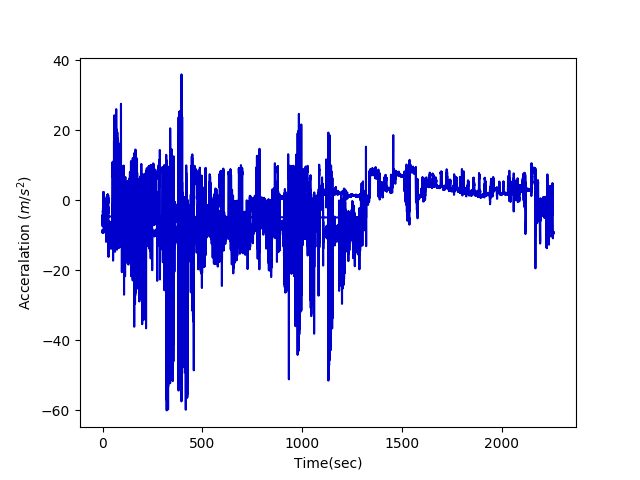
\includegraphics[width=.4\textwidth]{Figures/signal.png}
    \caption{Example of data coming from the x dimension of accelerator in the dataset for subject 1  }
    \label{fig:signal}
\end{figure}

As shown in Figure \ref{fig:signal}, the data coming from the sensors are scholastic over time and so as to extract the performed activities based on such signals, one of the Time-Series[TS] classification method should be applied. One of the best and widely used[] approach of TS classification is the sliding window process. This method consists of 5 steps which are shown in Figure \ref{fig:tsprocess} and are explained precisely in terms of HAR here.
\begin{itemize}
\item \textbf{Data acquisition:}There is a number of sensors attached to various parts of one's body which transform his or her the performing action to a set of signals and transmit them to the receiver(s). 
\item \textbf{Preprocesing:} The submitted data from sensors may be disrupted by different factors such as electronic fluctuations and in order to make it smooth there is varying kind of filtering process like the low-pass filter which was applied in some studies \cite{morris2014recofit}; although these filter may remove some valuable information from the signals.  
\item \textbf{Segmentation:}
As Figure \ref{fig:signal} indicates, there is a kind of motion in the signals and to capture it, the signals are partitioned into several parts (windows). The number of data points (window size) in each window heavily impacts the accuracy of classifiers and finding the best window size is very challenging and time-consuming. If each window shares some part of itself with the previous one, it is called overlapping sliding windowing.  

\item \textbf{Feature extraction:}
Then each window is transformed into a vector of features ranging from autocorrelation features \cite{morris2014recofit} to time/frequency domain [] and also statistical features to represent it.  
\item \textbf{Classification:}
Finally, the Machine Learning classifier is fed by the vector of features to train the extracted features and their labels and assigns the future observation to one of the learned activities or labels. 


\end{itemize}

% figure 2
\begin{figure}[h]
    \centering
    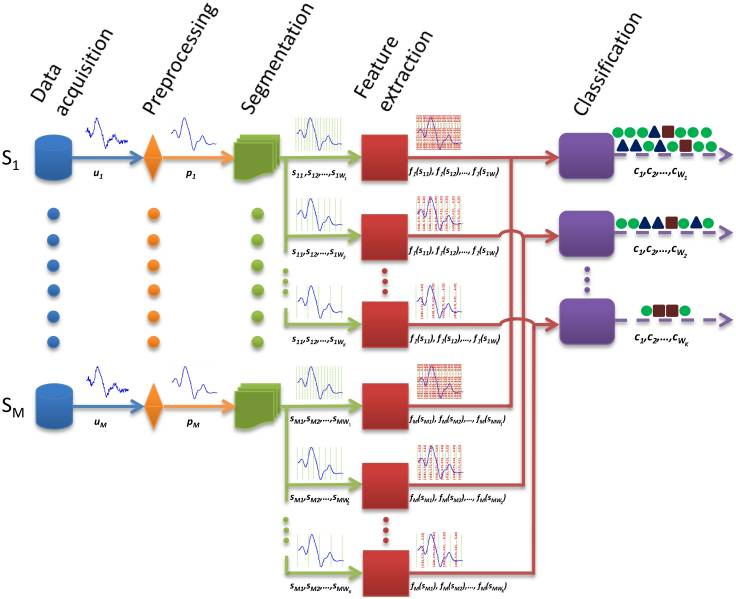
\includegraphics[width=.4\textwidth]{Figures/TSCprocess.jpeg}
    \caption{Time Series classification process through sliding window approach which is retrieved from \cite{banos2014window}}
    \label{fig:tsprocess}
\end{figure}



\section{Experiment setting}

\subsection{Dataset} \label{sec:dataset}
It is very important to use an adequate representative dataset to evaluate the impact of window size on the performance of the classifier in the recognition process. In this paper, one of the most complete human activity recognition dataset \cite{banos2012benchmark} in terms of the number of considered activities and subjects is used. This dataset is composed of data collected from 17 subjects of diverse profiles while wearing 9 Xsens inertial measurement units on different parts of their body and perform 33 fitness activities [Table \ref{tab:Activites}] ranging from Warm up to fitness exercises in an out-of-lab environment. Each sensor node provides tri-directional acceleration, gyroscope, and magnetic field
measurements as well as orientation estimates in quaternion format (4D). Although using several sensors help to capture the body dynamics, here only the acceleration data is used to study. This dataset provides data for three sensor displacement scenarios to compare the sensor anomalies(out of the scope of this work); thus, only the data from default scenario is used.

%  start of Table1
\begin{table}[h!]
\tiny  
  \centering
\begin{tabular}{|c|c|}
\hline 
\multicolumn{2}{|c|}{Activities}\tabularnewline
\hline 
\hline 
Walking (1 min) & Upper trunk and lower body opposite twist (20x)\tabularnewline
\hline 
Jogging (1 min) & Arms lateral elevation (20x)\tabularnewline
\hline 
Running (1 min) & Arms frontal elevation (20x)\tabularnewline
\hline 
Jump up (20x) & Frontal hand claps (20x)\tabularnewline
\hline 
Jump front \& back (20x) & Arms frontal crossing (20x)\tabularnewline
\hline 
Jump sideways (20x) & Shoulders high amplitude rotation (20x)\tabularnewline
\hline 
Jump leg/arms open/closed (20x) & Shoulders low amplitude rotation (20x)\tabularnewline
\hline 
Jump rope (20x) & Arms inner rotation (20x)\tabularnewline
\hline 
Trunk twist (arms outstretched) (20x) & Knees (alternatively) to the breast (20x)\tabularnewline
\hline 
Trunk twist (elbows bended) (20x) & Heels (alternatively) to the backside (20x)\tabularnewline
\hline 
Waist bends forward (20x) & Knees bending (crouching) (20x)\tabularnewline
\hline 
Waist rotation (20x) & Knees (alternatively) bend forward (20x)\tabularnewline
\hline 
Waist bends (reach foot with opposite hand) (20x) & Rotation on the knees (20x)\tabularnewline
\hline 
Reach heels backwards (20x) & Rowing (1 min)\tabularnewline
\hline 
Lateral bend (10x to the left + 10x to the right) & Elliptic bike (1 min)\tabularnewline
\hline 
Lateral bend arm up (10x to the left + 10x to the right) & Cycling (1 min)\tabularnewline
\hline 
Repetitive forward stretching (20x) & \tabularnewline
\hline 
\end{tabular}

      % Title of the table
        \caption{Activity set }
        \label{tab:Activites}

\end{table} 

%  end of Table1

\subsection{Setup}
In this section, the applied setups for activity recognition process which was explained in section {"if we add a section to explain the classification, it should be referred here"} are described. Regarding the prepossessing step, in order to avoid the removal of relevant information, here no prepossessing of the data is applied. As for segmentation,the overlapping (  sliding at 200ms i.e., each 5s window
shares 4.8s of data with the previous window) \cite{morris2014recofit} and non-overlapping \cite{banos2014window} sliding window approach with diverse window sizes ranging from .25 s to 7 s in the steps of .25 s are applied which this range covers most of the window sizes were used in previous studies[]. Although we believe that the non-overlapping sliding window approach overlooks some valuable patterns of movements between close windows, here it uses for the sake of comparison. 
In feature extraction part, three different feature sets(FS) are used namely FS1 = {mean}, FS2 ={mean and standard deviation} and FS3 = {mean, standard deviation, maximum, minimum and mean crossing rate}.Most of these features have been used in previous works[] due to their speed in the calculation and being informative over each window. Finally in recognition part, several powerful and common machine learning models are selected for discrimination of activities: Decision Tree (DT),k-nearest neighbors(KNN), Naive Bayes (NB), Nearest centroid classifier (NCC), Random forest(RF)and Logistic regression classifier(LR).We used these classifiers as implemented in scikit-learn 0.20 \cite{pedregosa2011scikit}.\newline
Here, a cross-validation (CV) process which according to \cite{arlot2010survey} is the most accurate approach for model selection is used in order to compare the performance of diverse models under different window size. However, due to the fact that data coming from sensors are temporal, we introduce two more realistic and promising cross-validation process which will be explained deeply in the next section.\newline
As can be seen in Figure \ref{fig:class}, the dataset is extremely imbalance meaning that there are more data-points for some classes(activities)in the dataset. Under such circumstances, the f1-score which conveys the balance between the precision and the recall based on the {} is an appropriate metric for evaluating the performance of the models. It reaches its best value at 1 (perfect precision and recall) and worst at 0.

% figure 2
\begin{figure}[h]
    \centering
    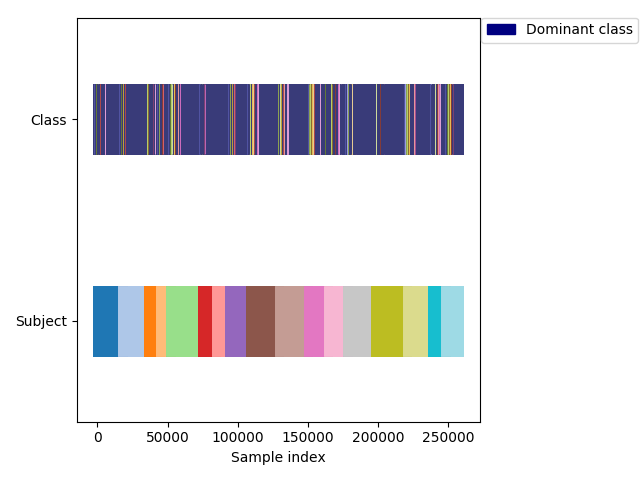
\includegraphics[width=.4\textwidth]{Figures/Class_subject.png}
    \caption{Example of distribution of activities and subjects in overlapping windowed dataset with window size=.5 s.The class 0 which means doing nothing accounts for more than 72 percent of the classes   }
    \label{fig:class}
\end{figure}

\subsection{Time Series  vs. Classic Cross-Validation}
In this section, different type of Cross-Validation(CV) strategies are explained and the reason that why classic CV is not suitable for activity recognition process.\newline

\begin{itemize}
\item \textbf{Classic Cross-validation}: The main hypothesis of this type of CV is that samples are Independent and Identically Distributed (i.i.d.).It means that all the data points sampled from the same distribution and also the distribution has no memory of past generated samples \ref{''}. Under such an assumption, as shown in Figure \ref{fig:iid-cv} the test set can be any part of the dataset. However, we know that samples coming from sensors are characterized to have correlation and the i.i.d. assumption of the CV is violated. Thus, evaluation models through classic CV would result in an illogical choosing of test and training set since the test set can be before the training set which is unreasonable. Although one may claim that after partitioning the dataset into some windows based on the Markov chain \cite{gilks1995markov} they are i.i.d..However, through splitting the dataset by a window size, there is no guarantee to find the best number of samples to make a window completely independent of others. 

% figure 3
\begin{figure}[h]
    \centering
    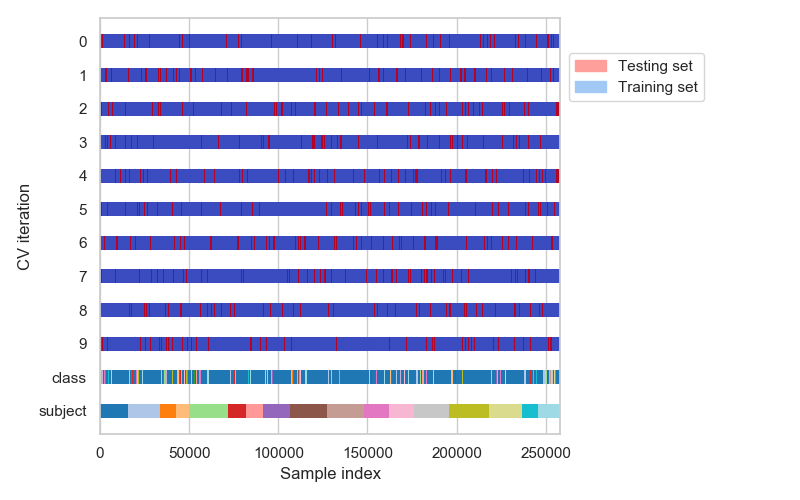
\includegraphics[width=.5\textwidth]{Figures/ShuffleSplit.png}
    \caption{10-CV process in overlapping windowed dataset by window size=.5 s }
    \label{fig:iid-cv}
\end{figure}


\item \textbf{Time-series Cross-validation:}
Due to the correlation between observations in Time-series based datasets, it is very crucial to train the model on the past samples and tests it on the future samples to estimate the generalization error of the trained model in the practice under a real-world scenario. As clearly illustrated in Figure \ref{fig:temporal-cv}, the Time-series CV focuses on splitting the dataset in such a way that the indices of the test set be higher than those of training set. It chooses the first K folds as training set and (K+1)-th as the test set. It should be noted that in each iteration the training sets are included the training sets that come before them. As an example in Figure \ref{fig:temporal-cv} the training set of fold \#3 includes training set \#2 and it includes \#1 and so on.
This method inspects how the models fare in the course of time.


% figure 3
\begin{figure}[h]
    \centering
    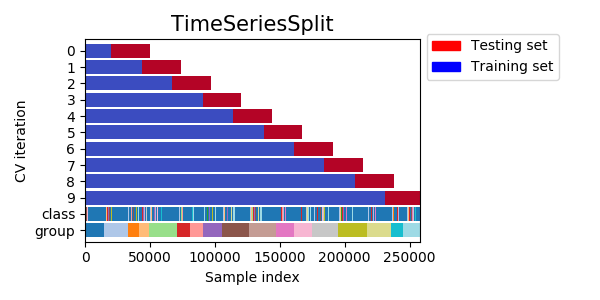
\includegraphics[width=.5\textwidth]{Figures/temporal-CV.png}
    \caption{10-TCV process in overlapping windowed dataset by window size=.5 s }
    \label{fig:temporal-cv}
\end{figure}

\item \textbf{Subjective Cross-validation:}
As mentioned before in section \ref{sec:dataset}, the used dataset in this study comprises the observations of 17 subjects with diverse profiles; consequently, such dataset is likely to be dependent on individual subjects. Under such circumstances, a safe approach to know the performance of the model is training on a particular set of subjects data and validate on the unseen ones in order to know how the trained model generalizes well on different groups. Although this method might be time-consuming (especially when the number of subjects is high), it is a very encouraging way to evaluate the domain-specific datasets. As can be seen in Figure \ref{fig:Subjective-cv}, in each fold the model trained on all groups except one which is used for testing.

% figure 4
\begin{figure}[h]
    \centering
    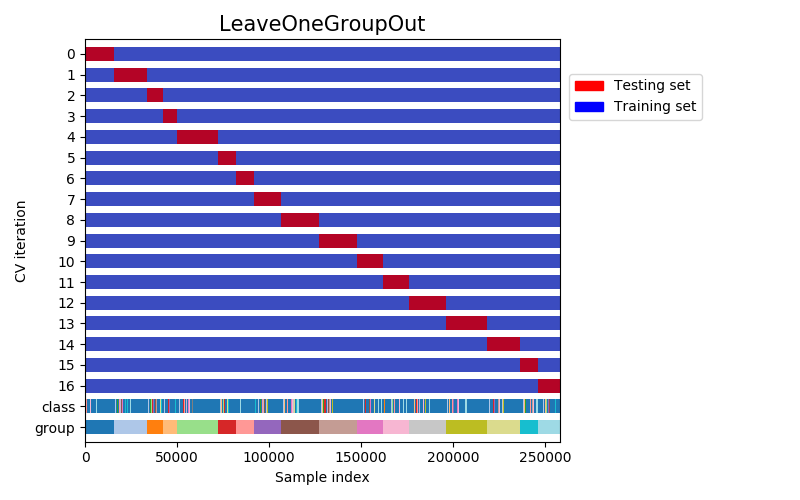
\includegraphics[width=.5\textwidth]{Figures/subjective-CV.png}
    \caption{17-SCV process in overlapping windowed dataset by window size=.5 s- here there are 17 subjects in the dataset,consequently 17 folds  }
    \label{fig:Subjective-cv}
\end{figure}

\end{itemize}





\section{Result}
Not Ready yet
\section{Discussion}



\section{Conclusions}
--------------------------
%\end{document}  % This is where a 'short' article might terminate




\begin{acks}

-----------
\end{acks}
